\chapter{Syntaktická a sémantická analýza kódu}
Abychom mohli implementovat náš jazyk (MonkeyC), je potřeba vytvořit aplikaci, která je schopna číst "věty" na vstupu a odpovídajicím způsobem rozpoznává klíčová slova či fráze naší gramatiky.(Obecně je jazyk složení platných vět, kdy věta se skládá z frází a fráze se skládá ze symbolů slovní zásoby).\\
Obecně lze říci, pokud nějaká aplikace vykonává (interpretuje) zápis jiného programu v jeho zdrojovém kódu ve zvoleném programovacím jazyce (v našem případě Typescript), že se jedná o tzv. interpret \cite{Interpret_2020}. Jako příklady je možné uvést kalkulačku, aplikace pro čtení konfiguračních souborů, Python interprety, atd... Pokud, na druhou stranu, dochází k převodu "věty" z jednoho jazyka do druhého (např. z Javy do 'C Sharp'), nazývá se taková aplikace překladačem.\\
Úkolem překladače či interpreta je tedy rozpoznat platné vstupy, tedy věty, fráze, subfráze, klíčová slova, atd... Přičemž rozpoznáním platného vstupu je myšleno identifikovat jednotlivé fráze a rozližit je od jiných.\\
Jako příklad použijeme rozpoznání vstupu $input = 1;$ s validní MonkeyC syntaxí. Syntaktický strom z těchto vstupních dat je možné vidět na obrázku \ref{img:assigment}. Z tohoto vstupu je patrné, že "input" je cíl přiřazení a "1" představuje hodnotu, která se má přiřadit. Stejně jako jsme my schopni rozližit v našem jazyce sloveso od podstatného jména, je naše aplikace schopna rozlišit toto přiřazení od např. importování knihovny pomocí klíčového slova "using".\\
Programy, které jsou schopny rozpoznávat konkrétní jazyk, se nazývají parsery nebo syntaktické analyzátory, přičemž syntax odkazuje na pravidla obsažená v popisu jazyka.\\

\begin{figure}[b!]
	\centering
	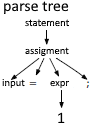
\includegraphics[scale=1.5]{images/assigment}
	 \caption{přiřazení hodnoty 1 proměnné input}
	 \label{img:assigment}
\end{figure}


\section{Parser a Lexer}
K vytvoření parseru a lexeru je potřeba spustit ANLTR nástroj, který na základě popisu jazyka (gramatiky) tyto souboru vygeneruje. S jejich pomocí je poté možné generovat syntaktické stromy pro vstupní data. Zde platí, že pokud jsou vstupní data validní (nejsou v rozporu s pravidly gramatiky), tak je vygenerovaný parser vždy rozpozná správně nehledě na složitost gramatiky.\\
Proces, při kterém dochází ke skládání znaků ze vstupních dat do slov či symbolů (tokenů) nese název \textbf{lexikální analýza} nebo \textbf{tokenizace}. Program, který provádí tuto tokenizaci se nazývá právě \textbf{lexer}. Obecně lze říci, že lexer (nebo také tokenizér) "rozdělí" text na vstupu (Monkey C kód) na tokeny. \cite{ANTLR_PG_20}. Dále lexer dokáže vytvořené tokeny seskupovat do tokenových tříd, nebo typů, např. IDENTIFIER (identifikátor), INTLITERAL (celočíselná proměnná), DOUBLELITERAL (proměnná typu double), atd...
V momentě, kdy lexer rozdělil vstupní data na jednotlivé tokeny, jsou tyto tokeny předány parseru. Ten poté "shora dolů" prochází text na vstupu a porovnává jednotlivé řádky s pravidly obsažené v gramatice \cite{ANTLR_PG_20}. Na obrázku \ref{img:parser} je možné vidět, jak parser zpracovává vstup $sp = 100;$. Tokeny, které lexer z těchto dat rozpozná, jsou [SP, =, 100, ;, <EOF>], kde SP je název proměnné, 100 hodnota, která je proměnné přiřazena, jako ve většině programovacích jazyků musí být příkaz ukončen středníkem, <EOF>, který se vyskytuje na konci každého validního vstupu, detekuje konec souboru (EOF - End Of File).


\begin{figure}[b!]
	\centering
	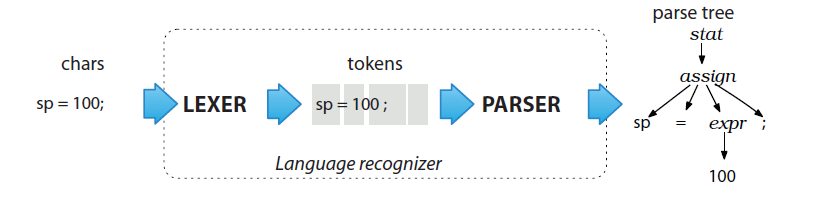
\includegraphics[scale=0.7]{images/parser}
	\caption{Ukázka, jak Language recognizer zpracovává vstupní sekvenci znaků} 			    \cite{ANTLR_PG_10}
	\label{img:parser}
\end{figure}

\section{Syntaktický strom}
Syntaktický strom představuje datovou strukturu, kterou ANTLR vytvoří při parsování vstupního souboru. Struktura je složená z kořene (root) a uzlů, které mohou představovat buď další podstromy, které odpovídají pravidlům gramatiky, nebo listy stromu.\\ 
V naší aplikaci Syntaktický strom představuje třída AST (viz. kód níže), která uchovává všechna důležitá data pro korektní analýzu vstupního souboru, např. počet uzlů stromu, soubor vztahující se ke konkrétnímu stromu, kořen stromu, atd...

\lstinputlisting[label=code:AST_TS,caption={třída AST v jazyce Typescript}]{SourceCodes/AST.tss}

Další, neméně důležitou, třídou v naší apikaci je třída Node, která představuje uzel stromu. Jedná se, ve své podstatě, o strukturu uchovávající následující atributy:\\
\begin{enumerate}
	\item kontext daného uzlu
	\item předka uzlu
	\item potomka uzlu
	\item hodnotu přestavující text v daném uzlu
	\item typ uzlu, který se odvíjí od pravidel v gramatice
\end{enumerate}

\lstinputlisting[label=code:Node_TS,caption={třída Node v jazyce Typescript}]{SourceCodes/Node.tss}


\section{ANTLR Listener a callback funkce}
ANTLR disponuje dvěma mechanismy, které umožňují průchod stromem (tzv. "tree-walking mechanisms"). Jedná se o mechanismy \textbf{listener} a \textbf{visitor},pričemž výchozím je listener. Největší rozdíl mezi nimi spočívá v tom, že listener metody jsou volány nezávisle ANTLR objektem, zatímco visitor metody vyvolávají rovněž metody potomků uzlu, na kterém se právě nachází, což způsobuje, že některé podstomy nebudou při průchodu vůbec navštíveny. Samotné listenery jsou ekvivalentí SAX objektům, které se používají v XML parserech.\\
Aby bylo možné stromem procházet a při průchodu vyvolat odpovídající události, ANTLR dispinuje třídou ParseTreeWalker. Právě ona se stará o to, aby byly volány callback funkce. Další důležitou komponentou, vygenerovanou ANTLR nástrojem je rozhraní ParseTreeListener (v našem případě MonkeyCListener \ref{img:generated_files}). Toto rozhraní definuje veškeré metody potřebné k kompletnímu průchodu stromem, např. "enterFunctionDeclaration(context: FunctionDeclarationContext)" či "exitFormalParameterDeclarations(context: FormalParameterDeclarationsContext)" \ref{img:listener_functions}. Ke každému pravidlu obsaženému v gramatice, parser vygeneruje 2 metody a kontextovou třídu. První metoda vždy začíná prefixem "enter" a druhá prefixem "exit", kontext poté odpovídá příslušnému pravidlu. Ve chvíli kdy ParseTreeWalker narazí na příslušný uzel, vyvolá odpovídající metodu, podle toho zda do uzlu vstupuje, nebo jej opouští.

\begin{figure}[t]
	\centering
	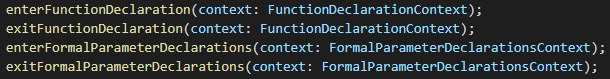
\includegraphics[scale=1]{images/listener_functions}
	\caption{funkce vygenerované nástrojem ANTLR} 			    
	\label{img:listener_functions}
\end{figure}

\endinput
